\documentclass[14pt, a4paper]{article}
\usepackage{minitoc}
\usepackage[left=3.00cm, right=2.5cm, top=2.00cm, bottom=2.00cm]{geometry}
\usepackage{amsmath}
\usepackage{amssymb}
\usepackage{amsthm}
\usepackage{mathrsfs}
\usepackage{thmtools}
\usepackage{mathtools}
\usepackage{graphicx}
%\usepackage{algpseudocode}
%\usepackage{algorithm}
\usepackage[ruled,vlined,linesnumbered,algosection]{algorithm2e}
\usepackage{blindtext}
\usepackage{setspace}
\usepackage[utf8]{inputenc}
\usepackage[utf8]{vietnam}
\usepackage[center]{caption}
\usepackage[shortlabels]{enumitem}
\usepackage{fancyhdr} % header, footer
\usepackage{hyperref} % loại bỏ border với mục lục và công thức
\usepackage[nonumberlist, nopostdot, nogroupskip]{glossaries}
\usepackage{glossary-superragged}
\usepackage{tikz,tkz-tab}
\setglossarystyle{superraggedheaderborder}
\pagestyle{fancy}
%\usepackage[style=numeric,sortcites]{biblatex}
%\addbibresource{ref.bib}
%\usepackage[numbers]{natbib}
\usepackage{indentfirst}
\usepackage{multirow}
\usepackage[natbib,backend=biber,style=ieee, sorting=ynt]{biblatex}
\usepackage{cancel}
\bibliography{ref.bib}

\graphicspath{{./figures/}}


\hypersetup{
    colorlinks=false,
    pdfborder={0 0 0},
}


\fancyhf{}
\rhead{\textbf{Môn học: Các phương pháp ngẫu nhiên và ứng dụng}}
\lhead{\textbf{GVHD: PGS. TS. Tạ Công Sơn}}
\rfoot{\thepage}
\lfoot{\textbf{Học viên thực hiện: Nguyễn Chí Thanh - 21007925}}
\renewcommand{\headrulewidth}{0.4pt}
\renewcommand{\footrulewidth}{0.4pt}


\numberwithin{equation}{section}
\numberwithin{figure}{section}

\setlength{\parindent}{0.5cm}

\setcounter{secnumdepth}{3} % Cho phép subsubsection trong report
\setcounter{tocdepth}{3} % Chèn subsubsection vào bảng mục lục

\newtheorem{md}{Mệnh đề}

\newtheorem{dl}{Định lý}
\newtheoremstyle{sltheorem}
{}                % Space above
{}                % Space below
{\normalfont}        % Theorem body font % (default is "\upshape")
{}                % Indent amount
{\bfseries}       % Theorem head font % (default is \mdseries)
{.}               % Punctuation after theorem head % default: no punctuation
{ }               % Space after theorem head
{}                % Theorem head spec
\theoremstyle{sltheorem}
\newtheorem{vd}{Ví dụ}
\newtheoremstyle{soltheorem}
{}                % Space above
{}                % Space below
{\normalfont}        % Theorem body font % (default is "\upshape")
{}                % Indent amount
{\bfseries}       % Theorem head font % (default is \mdseries)
{.}               % Punctuation after theorem head % default: no punctuation
{\newline}               % Space after theorem head
{}                % Theorem head spec
\theoremstyle{soltheorem}
\newtheorem*{loigiai}{Lời giải}

\numberwithin{dl}{section}
\numberwithin{md}{section}
\numberwithin{vd}{section}

\doublespacing

\begin{document}
    \begin{titlepage}

        \newcommand{\HRule}{\rule{\linewidth}{0.5mm}} % Defines a new command for the horizontal lines, change thickness here

        \center % Center everything on the page

        %----------------------------------------------------------------------------------------
        %	HEADING SECTIONS
        %----------------------------------------------------------------------------------------
        \textsc{\LARGE Đại học Quốc Gia Hà Nội}\\[0.5cm]
        \textsc{\LARGE Trường đại học Khoa học tự nhiên}\\[0.5cm] % Name of your university/college
        \textsc{\LARGE Khoa Toán - Cơ - Tin học}\\[0.5cm]

        
\includegraphics[scale=0.2]{HUS-logo.jpg}\\[0.5cm]

        \textsc{\Large Chuyên ngành: Khoa học dữ liệu}\\[0.5cm] % Major heading such as course name


        %----------------------------------------------------------------------------------------
        %	TITLE SECTION
        %----------------------------------------------------------------------------------------

        \HRule \\[0.4cm]
        { \huge \bfseries TIỂU LUẬN MÔN HỌC}\\[0.4cm] % Title of your document
        \HRule \\[1.5cm]

        \textsc{\Large Môn học: Các phương pháp ngẫu nhiên và ứng dụng}\\[1cm] % Minor heading such as course title


        \textsc{\Large Đề tài: Xích Markov và Lý thuyết phân nhánh}\\[2cm]


        %----------------------------------------------------------------------------------------
        %	AUTHOR SECTION
        %----------------------------------------------------------------------------------------
        \begin{minipage}{0.4\textwidth}
            \begin{flushleft} \large
            \emph{Giảng viên hướng dẫn:} \\
            PGS. TS. Tạ Công Sơn % Supervisor's Name
            \end{flushleft}
        \end{minipage}\\[0.5cm]

        \begin{minipage}{0.4\textwidth}
        \begin{flushleft} \large
        \emph{Học viên thực hiện:}\\
        Nguyễn Chí Thanh \\
        MSHV: 21007925 \\ % Your name
        Lớp: Khoa học dữ liệu - K4
        \end{flushleft}
        \end{minipage}


        % If you don't want a supervisor, uncomment the two lines below and remove the section above
        %\Large \emph{Author:}\\
        %John \textsc{Smith}\\[3cm] % Your name

        %----------------------------------------------------------------------------------------
        %	DATE SECTION
        %----------------------------------------------------------------------------------------

        % I don't want day because it is English
        % {\large \today}\\[2cm] % Date, change the \today to a set date if you want to be precise

        %----------------------------------------------------------------------------------------
        %	LOGO SECTION
        %----------------------------------------------------------------------------------------

        %\includegraphics{logo/rsz_3logo-khtn.png}\\[1cm] % Include a department/university logo - this will require the graphicx package

        %----------------------------------------------------------------------------------------

        \vfill % Fill the rest of the page with whitespace

    \end{titlepage}

    \cleardoublepage
    \pagenumbering{gobble}
    \tableofcontents
    \newpage
    \listoffigures
    \newpage
    \glsaddall 
    \renewcommand*{\glossaryname}{Danh mục các từ viết tắt}
    \renewcommand*{\acronymname}{Danh sách từ viết tắt}
    \renewcommand*{\entryname}{Viết tắt}
    \renewcommand*{\descriptionname}{Viết đầy đủ}
    \printnoidxglossary
    \cleardoublepage
    \pagenumbering{arabic}

    %\maketitle

    \newpage

    \nocite{*}

    \begin{center}
    \section*{LỜI MỞ ĐẦU}
    \end{center}
    \addcontentsline{toc}{section}{{\bf LỜI MỞ ĐẦU}\rm}

    \newpage

    \section{Số bước trung bình chuyển tiếp giữa các trạng thái tạm thời}

    Ta xét một xích Markov trạng thái hữu hạn và giả định rằng các trạng thái được đánh số $T=\lbrace 1, 2, \dots, t \rbrace$ ký hiệu tập các trạng thái tạm thời.
    Ta đặt:

    \begin{equation*}
        \mathbf{P}_T = \begin{bmatrix} P_{11} & P_{12} & \dots & P_{1t} \\ \vdots & \vdots & \vdots & \vdots \\ P_{t1} & P_{t2} & \dots & P_{tt}  \end{bmatrix}
    \end{equation*}

    Và ta cần chú ý rằng ma trận $\mathbf{P}_T$ chỉ xác định xác suất chuyển tiếp từ các trạng thái tạm thời sang trạng thái tạm thời, và tổng của một số hàng nhỏ hơn 1 (mặt khác $T$ có thể là một tập đóng của các trạng thái).
    
    Ta xét hai trạng thái tạm thời $i$ và $j$, ta đặt $s_{ij}$ ký hiệu là số bước kỳ vọng mà xích Markov đến trạng thái $j$, khi ta biết xích Markov bắt đầu ở trạng thái $i$.
    Đặt $\delta_{i,j}=1$ khi $i=j$ và bằng 0 nếu ngược lại.
    Ta tính $s_{ij}$ sử dụng công thức kỳ vọng đầy đủ:

    \begin{equation} \label{eq:expected_number_periods_i_to_j}
        \begin{aligned}
            s_{ij} &= \delta_{i,j} + \sum_{k \in T} P_{ik}s_{kj} \\
            &= \delta_{i,j} + \sum_{k=1}^t P_{ik} s_{kj}
        \end{aligned}
    \end{equation}

    với đẳng thức cuối cùng của công thức trên cho ta thấy không thể chuyển từ một trạng thái hồi quy sang một trạng thái tạm thời, ý nghĩa rằng $s_{kj}=0$ khi $k$ là một trạng thái hồi quy.

    Ta đặt $\mathbf{S}$ ký hiệu là ma trận với các giá trị $s_{ij}, i, j = 1, \dots, t$. Ta có ma trận $\mathbf{S}$:

    \begin{equation*}
        \mathbf{S} = \begin{bmatrix} s_{11} & s_{12} & \dots & s_{1t} \\ \vdots & \vdots & \vdots & \vdots \\ s_{t1} & s_{t2} & \dots & s_{tt}  \end{bmatrix}
    \end{equation*}

    Ta viết lại công thức \ref{eq:expected_number_periods_i_to_j} dưới dạng ma trận:

    \begin{equation*}
        \mathbf{S} = \mathbf{I} + \mathbf{P}_T \mathbf{S}
    \end{equation*}

    với $\mathbf{I}$ là ma trận đơn vị kích thước $t$. Bởi vì công thức trên tương đương với:

    \begin{equation*}
        (\mathbf{I} - \mathbf{P}_T) \mathbf{S} = \mathbf{I}
    \end{equation*}

    Bằng cách nhân cả hai vế với $(\mathbf{I} - \mathbb{P}_T)^{-1}$ ta thu được:

    \begin{equation*}
        \mathbf{S} = (\mathbf{I} - \mathbf{P}_T)^{-1}
    \end{equation*}

    Với mỗi đại lượng $s_{ij}, i \in T, j \in T$, ta có thể tính đại lượng này bằng cách lấy phần tử tại hàng $i$ và cột $j$ của ma trận nghịch đảo của ma trận $\mathbf{I} - \mathbf{P}_T$ (sự tồn tại của ma trận nghịch đảo này dễ dàng chứn minh được).

    \begin{vd} \label{vd:gambler-ruin-problem}
        Ta xét bài toán người đánh bạc với $p=0.4$ và $N=7$. Bắt đầu với 3 đô la, xác định:
        \begin{enumerate}[label=(\alph*)]
            \item Số ván kỳ vọng để người chơi bài có 5 đô la.
            \item Số ván kỳ vọng để người chơi bài có 2 đô la.
        \end{enumerate}
    \end{vd}

    \begin{loigiai}
        Ma trận $\mathbf{P}_T$ xác định các giá trị $P_{ij}, i, j \in \lbrace 1, 2, 3, 4, 5, 6 \rbrace$ được xác định như sau:

        \begin{equation*}
            \mathbf{P}_T = \begin{bmatrix}
                0 & 0.4 & 0 & 0 & 0 & 0 \\
                0.6 & 0 & 0.4 & 0 & 0 & 0 \\
                0 & 0.6 & 0 & 0.4 & 0 & 0 \\
                0 & 0 & 0.6 & 0 & 0.4 & 0 \\
                0 & 0 & 0 & 0.6 & 0 & 0.4 \\
                0 & 0 & 0 & 0 & 0.6 & 0 \\
            \end{bmatrix}
        \end{equation*}

        Ta tính nghịch đảo ma trận $\mathbf{I} - \mathbf{P}_T$, ta thu được:

        \begin{equation*}
            \mathbf{S}=(\mathbf{I}-\mathbf{P}_T)^{-1}=
            \begin{bmatrix}
            1.6149 & 1.0248 & 0.6314 & 0.3691 & 0.1943 & 0.0777 \\
            1.5372 & 2.5619 & 1.5784 & 0.9228 & 0.4857 & 0.1943 \\
            1.4206 & 2.3677 & 2.9990 & 1.7533 & 0.9228 & 0.3691 \\
            1.2458 & 2.0763 & 2.6299 & 2.9990 & 1.5784 & 0.6314 \\
            0.9835 & 1.6391 & 2.0763 & 2.3677 & 2.5619 & 1.0248 \\
            0.5901 & 0.9835 & 1.2458 & 1.4206 & 1.5372 & 1.6149
            \end{bmatrix}
        \end{equation*}

        Vì vậy ta thu được $s_{3,5}=0.9228$ (ván) và $s_{3,2}=2.3677$ (ván).
    \end{loigiai}

    Với $i \in T, j \in T$, đại lượng $f_{ij}$ chính là xác suất để để xích Markov tạo ra một quỹ đạo chuyển tiếp đạt đến trạng thái $j$ khi biết xích Markov bắt đầu từ trạng thái $i$ dễ dàng được xác định từ $\mathbf{P}_T$.
    Để xác định mối liên hệ, ta bắt đầu từ biệc sử dụng công thức tính $s_{ij}$ dựa trên hệ đầy đủ là xích Markov đã từng đi qua trạng thái $j$ hay chưa.
    Sử dụng công thức kỳ vọng đầy đủ ta thu được:

    \begin{equation*}
        \begin{aligned}
            s_{ij} &= E \lbrack \text{ số bước để đến được } j \vert \text{ bắt đầu tại } i, \text{ đã từng đi qua } j \rbrack f_{ij} \\ & + E \lbrack \text{ số bước để đến được } j \vert \text{ bắt đầu tại } i, \text{ chưa từng đi qua } j \rbrack (1 - f_{ij}) \\
            &= (\delta_{i, j} + s_{{jj}}) f_{ij} + \delta_{ij}(1 - f_{ij}) \\
            &= \delta_{i,j} + f_{ij} s_{jj}
        \end{aligned}
    \end{equation*}

    với $s_{jj}$ là số bước kỳ vọng cần thêm vào khi trạng thái $j$ đã đạt và tiếp tục một lần nữa quay lại trạng thái $j$.
    Giải phương trình trên ta thu được:

    \begin{equation*}
        f_{ij} = \dfrac{s_{ij} - \delta_{i,j}}{s_{jj}}
    \end{equation*}

    \begin{vd}
        Trong ví dụ \ref{vd:gambler-ruin-problem}, xác suất là bao nhiêu để người chơi có lúc có 1 đô la?
    \end{vd}

    \begin{loigiai}
        Với $s_{31}=1.4206$ và $s_{11}=1.6149$, ta thu được:
        
        \begin{equation*}
            f_{31} = \dfrac{s_{31}}{s_{11}}=0.8797
        \end{equation*}

        Để kiểm tra lại, ta chú ý rằng $f_{31}$ chính là xác suất người đánh bạc bắt đầu với 3 đô la và có 1 đô la trước khi đạt được 7 đô la.
        Đây chính là xác suất để người đánh bạc mất 2 đô la trước khi có thêm 4 đô la cũng bằng xác suất người đánh bạc bắt đầu với 2 đô la và thu cuộc trước khi đạt được 6 đô la.
        Vì vậy:

        \begin{equation*}
            f_{31} = - \dfrac{1 - (0.6/0.4)^2}{1-(0.6/0.4)^6}=0.8797
        \end{equation*}
        và kết quả trùng khớp với cách làm đầu tiên.
    \end{loigiai}

    Giả sử ta đang quan tâm đến số bước kỳ vọng để xích Markov đi đến một tập các trạng thái $A$, không nhất thiết phải là các trạng thái lặp lại.
    Ta có thể giả định về tình huống trước bằng cách làm cho tất cả các trạng thái trong $A$ là trạng thái hấp thụ bằng cách đặt lại xác suất chuyển tiếp của các trạng thái trong tập $A$ thỏa mãn:
    \begin{equation*}
        P_{ii} = 1, i \in A
    \end{equation*}

    Việc này biến các trạng thái trong tập $A$ thành trạng thái hồi quy, và biến đổi bất kỳ trạng thái nào ngoài tập $A$ nhưng cuối cùng cũng chuyển tiếp vào một trạng thái trong tập $A$ thành một trạng thái tạm thái.
    Vì vậy, cách tiếp cận trước đây của ta có thể được sử dụng
    
    \section{Các quá trình phân nhánh}
    
    Trong phần này ta sẽ xem xét một lớp các xích Markov được gọi là các \textit{quá trình phân nhánh}.
    Lớp xích Markov này có ứng dụng rất rộng rãi trong y học, xã hội học và khoa học kỹ thuật.
    
    Ta xét một quần thể bao gồm các cá thể có thể tạo ra các thế hệ tiếp theo cùng loài.
    Ta giả định rằng từng cá thể đến cuối thời gian sống tạo ra $j$ con với xác suất $P_j, j \geq 0$ và độc lập với số con được sinh ra bởi cá thể khác.
    Ta giả sử $P_j < 1 \forall j \geq 0$.
    Số cá thể ban đầu được ký hiệu là $X_0$, được gọi là kích cỡ của thế hệ thứ 0.
    Tất cả con cháu của thế hệ thứ 0 tạo thành thế hệ đầu tiên và kích thước của quần thể tại thế hệ này ký hiệu là $X_1$.
    Tổng quát, ta đặt $X_n$ ký hiệu là kích cỡ của thế hệ thứ $n$.
    Vì vậy $\lbrace X_n \rbrace_{n=0,1,\dots}$ là một xích Markov có không gian trạng thái là tập hợp các số nguyên không âm.
    
    Ta cần chú ý rằng trạng thái 0 là một trạng hồi quy, vì rõ ràng $P_{00}=1$.
    Ngoài ra nếu $P_0 > 0$, tất cả các trạng thái khác là trạng thái tạm thời.
    Điều này xảy ra khi $P_{i0}=P_0^i$ có ý nghĩa quần thể ban đầu có $i$ cá thể và có xác suất ít nhất $P_0^i$ sẽ không còn thế hệ nào nữa mà quần thể bao gồm $i$ cá thể.
    Hơn nữa, vì bất kỳ tập hữu hạn các trạng thái tạm thời $\lbrace 1, 2, \dots, n \rbrace$ sẽ được xích Markov đi qua một số hữu hạn lần, dẫn đến một kết luận quan trọng là nếu $P_0 > 0$, số lượng quần thể sẽ về 0 hoặc tiến đến vô cùng.
    
    Ta đặt:
    \begin{equation*}
        \mu = \sum_{j=0}^{\infty} j P_j
    \end{equation*}
    
    ký hiệu số các con trung bình do một cá thể sinh ra và đặt:
    \begin{equation*}
        \sigma^2 = \sum_{j=0}^{\infty} (j - \mu)^2 P_j
    \end{equation*}
    là phương sai của số các con được tạo ra bởi một cá thể.
    
    Ta giả định rằng $X_0 = 1$, ban đầu chỉ có duy nhất 1 cá thể.
    Ta tính $E \lbrack X_n \rbrack$ và $\mathrm{Var} (X_n)$, ta có thể viết:
    \begin{equation*}
        X_n = \sum_{i=1}^{X_n - 1} Z_i
    \end{equation*}

    với $Z_i$ biểu diễn số con cháu ở cá thể thứ $i$ của thế hệ thứ $n-1$.
    Ta tính kỳ vọng của $X_n$ bằng cách lấy điều kiện trên $X_{n-1}$, ta thu được:

    \begin{equation*}
        \begin{aligned}
            E \lbrack X_n \rbrack &= E \lbrack E \lbrack X_n \vert X_{n-1} \rbrack \rbrack \\
            &= E \Bigg \lbrack E \Bigg \lbrack \sum_{i=1}^{X_n - 1} Z_i \vert X_{n-1} \Bigg \rbrack \Bigg \rbrack \\
            &= E \lbrack X_{n-1} \mu \rbrack \\
            &= \mu E \lbrack X_{n-1} \rbrack
        \end{aligned}
    \end{equation*}

    ta sử dụng $E \lbrack Z_i \rbrack = \mu$. Vì $E \lbrack X_0 \rbrack = 1$, công thức trên trở thành:

    \begin{equation*}
        \begin{aligned}
            E \lbrack X_1 \rbrack &= \mu \\
            E \lbrack X_2 \rbrack &= \mu E \lbrack X_1 \rbrack = \mu^2 \\
            & \vdots \\
            E \lbrack X_n \rbrack &= \mu E \lbrack X_{n-1} \rbrack = \mu^n
        \end{aligned}
    \end{equation*}

    Tương tự, $\mathrm{Var} (X_n)$ có thể được tính sử dụng công thức phương sai có điều kiện:

    \begin{equation*}
        \mathrm{Var} (X_n) = E \lbrack \mathrm{Var} (X_n \vert X_{n-1}) \rbrack + \mathrm{Var} (E \lbrack X_n \vert X_{n-1} \rbrack)
    \end{equation*}

    Khi ta đã biết $X_{n-1}$, $X_n$ là tổng của $X_{n-1}$ biến ngẫu nhiên độc lập có phân bố $\lbrace P_j, j \geq 0 \rbrace$.
    Vì vậy:

    \begin{equation*}
        E \lbrack X_n \vert X_{n-1} \rbrack = X_{n-1} \mu, \mathrm{Var} (X_n \vert X_{n-1}) = X_{n-1} \sigma^2
    \end{equation*}

    Công thức phương sai có điều kiện bây giờ trở thành:

    \begin{equation*}
        \begin{aligned}
            \mathrm{Var}(X_n) & =E[X_{n-1} \sigma^2]+\mathrm{Var}(X_{n-1} \mu) \\
            &=\sigma^2 \mu^{n-1}+\mu^2 \mathrm{Var}(X_{n-1}) \\
            &=\sigma^2 \mu^{n-1}+\mu^2(\sigma^2 \mu^{n-2}+\mu^2 \mathrm{Var}(X_{n-2})) \\
            &=\sigma^2(\mu^{n-1}+\mu^n)+\mu^4 \mathrm{Var}(X_{n-2}) \\
            &=\sigma^2(\mu^{n-1}+\mu^n)+\mu^4(\sigma^2 \mu^{n-3}+\mu^2 \mathrm{Var}(X_{n-3})) \\
            &=\sigma^2(\mu^{n-1}+\mu^n+\mu^{n+1})+\mu^6 \mathrm{Var}(X_{n-3}) \\
            &=\cdots \\
            &=\sigma^2(\mu^{n-1}+\mu^n+\cdots+\mu^{2 n-2})+\mu^{2 n} \mathrm{Var}(X_0) \\
            &=\sigma^2(\mu^{n-1}+\mu^n+\cdots+\mu^{2 n-2})
        \end{aligned}
    \end{equation*}

    Vì vậy,

    \begin{equation}
        \begin{aligned}
            \mathrm{Var} (X_n) = \begin{cases}
                \sigma^2 \mu^{n-1} \Big ( \dfrac{1 - \mu^n}{1 - \mu} \Big) &\text{ nếu } \mu \neq 1 \\
                n \sigma^2 &\text{ nếu } \mu = 1
            \end{cases}
        \end{aligned}
    \end{equation}

    Ta đặt $\pi_0$ ký hiệu quần thể cuối cùng sẽ biến mất (với giả định là $X_0=1$). Về mặt hình thức:

    \begin{equation*}
        \pi_0 = \lim_{n \rightarrow \infty} P \lbrace X_n = 0 \vert X_0 = 1 \rbrace
    \end{equation*}

    Bài toán xác định giá trị $pi_0$ lần đầu tiên được đặt ra bởi Galton vào năm 1889 liên quan tới sự biến mất của một dòng họ.

    Ta thấy rằng $pi_0 = 1$ nếu $\mu < 1$ vì:

    \begin{equation*}
        \begin{aligned}
            \mu^n = E \lbrack X_n \rbrack &= \sum_{j=1}^{\infty} j P \lbrace X_n = j \rbrace \\
            & \geq \sum_{j=1}^{\infty} 1. P \lbrace X_n = j \rbrace \\
            & = P \lbrace X_n \geq 1 \rbrace
        \end{aligned}
    \end{equation*}

    Ta nhận thấy $\mu^n \rightarrow 0$ khi $\mu < 1$ kéo theo $P \lbrace X \geq 1 \rbrace \rightarrow 0$ vì vậy $P \lbrace X_n = 0 \rbrace \rightarrow 1$.

    Thực tế, ta có thể chỉ ra $\pi_0 = 1$ ngay cả khi $\mu = 1$.K
    Khi $\mu > 1$, ta thấy $\pi_0 < 1$, và công thức xác định $p_0$ nhận được bằng cách lấy điều kiện trên số con cháu của từng cá thể trong quần thể tại thế hệ 0:

    \begin{equation*}
        \begin{aligned}
            \pi_0 &= P \lbrace \text{quần thể biến mất} \rbrace \\
            &= \sum_{j=0}^{\infty} P \lbrace \text{quần thể biến mất} \vert X_1 = j \rbrace P_j
        \end{aligned}        
    \end{equation*}

    Bây giờ, khi biết $X_1 = j$, quần thể sẽ bị biến mất khi và chỉ khi nếu từng dòng họ trong $j$ dòng họ được bắt đầu bằng các cá thể của thế hệ thứ nhất biến mất.
    Ta giả sử từng dòng họ hoạt động độc lặp vì vậy, xác suất để từng dòng họ bị biến mất là $\pi_0$, ta thu được:
    
    \begin{equation*}
        P \lbrace \text{quần thể biến mất}\vert X_1 = j \rbrace = \pi_0^j
    \end{equation*}

    và $\pi_0$ thỏa mãn:

    \begin{equation} \label{eq:pi_0}
        \pi_0 = \sum_{j=0}^{\infty} \pi_0^j P_j
    \end{equation}

    Thực tế khi $\mu > 1$, ta có thể thấy $\pi_0$ là số dương nhỏ nhất thỏa mãn công thức \ref{eq:pi_0}.

    \begin{vd}
        Nếu $P_0 = \dfrac{1}{2}, P_1 = \dfrac{1}{4}, P_2 = \dfrac{1}{4}$. Xác định $\pi_0$
    \end{vd}

    \begin{loigiai}
        Vì $\mu = \dfrac{3}{4} \leq 1$ nên $\pi_0 = 1$
    \end{loigiai}

    \begin{vd} \label{vd:4.32}
        Nếu $P_0 = \dfrac{1}{4}, P_1 = \dfrac{1}{4}, P_2 = \dfrac{1}{2}$. Xác định $\pi_0$.
    \end{vd}

    \begin{loigiai} \label{vd:4.33}
        $\pi_0$ thỏa mãn:
        \begin{equation*}
            \pi_0 = \dfrac{1}{4} + \dfrac{1}{4} \pi_0 + \dfrac{1}{2} \pi_0^2
        \end{equation*}

        hoặc

        \begin{equation*}
            2 \pi_0^2 - 3 \pi_0 + 1 = 0
        \end{equation*}

        Nghiệm dương nhỏ nhất của phương trình bậc 2 này là $\pi_0 = \dfrac{1}{2}$
    \end{loigiai}

    \begin{vd}
        Trong ví dụ \ref{vd:4.32} và ví dụ \ref{vd:4.33}, xác suất cả quần thì bị biến mất là bao nhiêu nếu ban đầu bao gồm $n$ cá thể?
    \end{vd}

    \begin{loigiai}
        Khi cả quần thể bị biến mất khi và chỉ khi tất cả các dòng họ của từng thành viên của thế hệ ban đầu biến mất, xác suất này là $\pi_0^n$.
        Ví dụ \ref{vd:4.32} thu được $\pi_0^n = 1$, và cho ví dụ \ref{vd:4.33}, $\pi_0^n = \Big ( \dfrac{1}{2} \Big )^n$
    \end{loigiai}

    \section{Xích Markov đảo ngược thời gian}

    Ta xét một xích Markov ergodic dừng (là một xích Markov đã được vận hành một thời gian dài) có xác suất chuyển trạng thái $P_{ij}$ và phân bố dừng $\pi_i$ và ta giả sử rằng tại một vài thời điểm ta lưu vết dãy các trạng thái đi ngược thời gian.
    Bắt đầu ở thời điểm, ta xét dãy các trạng thái $X_n, X_{n-1}, X_{n-2}, \dots$.
    Ta nhận thấy dãy trạng thái này cũng là một xích Markov với xác suất chuyển trạng thái $Q_{ij}$ được định nghĩa bởi:

    \begin{equation*}
        \begin{aligned}
            Q_{ij} &= P \lbrace X_m = j \vert X_{m+1} = i \rbrace \\
            &= \dfrac{P \lbrace X_m = j, X_{m+1}=i \rbrace}{P \lbrace X_{m+1}=i \rbrace} \\
            &= \dfrac{P \lbrace X_m = j \vert X_{m+1} = i \rbrace P \lbrace X_{m+1=i \vert X_m = j \rbrace}}{P \lbrace X_{m+1}=j \rbrace} \\
            &= \dfrac{\pi_j P_{ji}}{\pi_i}
        \end{aligned}
    \end{equation*}

    Để chứng minh quá trình ngược thực sự là một xích Markov ta cần kiểm chứng:

    \begin{equation*}
        P \lbrace X_m = j \vert X_{m+1}=i, X_{m+2}, X_{m+3}, \dots \rbrace P \lbrace X_m = j \vert X_{m+1}=i \rbrace
    \end{equation*}

    Ta xét thời điểm hiện tại là $m+1$. Khi $X_0, X_1, X_2, \dots$ là một xích Markov, phân bố có điều kiện của các trạng thái tương lai $X_{m+2}, X_{m+3}, \dots$ khi cho trạng thái hiện tại $X_{m+1}$ độc lập vào trạng thái quá khứ $X_m$.
    Tuy nhiên, tính độc lập là một mối quan hệ đối xứng (nếu A độc lập với B thì B cũng độc lập với A) và vì vậy khi biết $X_{m+1}$ thì $X_m$ độc lập với $X_{m+2}, X_{m+3}, \dots$ và đây chính xác là việc ta cần kiểm chứng.

    Vì vậy, quá trình ngược cũng là một xích Markov với xác suất chuyển trạng thái được tính bởi công thức:

    \begin{equation*}
        Q_{ij} = \dfrac{\pi_j P_{ji}}{\pi_i}
    \end{equation*}

    Nếu $Q_{ij} = P_{ij}$ với mọi $i, j$ khi đó xích Markov được gọi là khả đảo thời gian.
    Điều kiện cho việc khả đảo thời gian $Q_{ij}=P_{ij}$ có thể được biểu diễn bởi:

    \begin{equation} \label{eq:Time-Reversible}
        \pi_i P_{ij} = \pi_j P_{ji} \forall i, j
    \end{equation}

    Điều kiện trong công thức \ref{eq:Time-Reversible} có thể được phát biểu là với mọi trạng thái $i$ và $j$, tỷ lệ quá trình đi từ $i$ đến $j$ ($\pi_i P_{ij}$) bằng với tỷ lệ quá trình đi từ $j$ đến $i$ ($\pi_j P_{ji}$).
    Một điều rất cần chú ý là điều kiện cần hiển nhiên cho tính khả đảo thời gian là chuyển tiếp từ $i$ đến $j$ khi đi ngược thời gian tương đương với chuyển tiếp từ $j$ sang $i$ khi đi theo thuận chiều thời gian.
    Nếu $Xm=i$ và $X_{m-1}=j$ thì một phép biến đổi từ $i$ sang $j$ được quan sát nếu ta quan sát ngược thời gian và một từ $j$ sang $i$ nếu ta nhìn thuận chiều thời gian.
    Vì vậy, tỷ lệ mà quá trình thuận tạo ra một chuyên tiếp từ $j$ sang $i$ luôn luôn bằng với tỷ lệ quá trình ngược tạo ra một chuyển tiếp từ $i$ sang $j$.
    Nếu khả đảo thời gian, tỷ lệ tạo ra một chuyển trạng thái từ $i$ sang $j$ của quá trình thuận và quá trình ngược phải bằng nhau.

    Nếu ta có thể tìm các số không âm, tổng bằng 1 và thỏa mãn phương trình \ref{eq:Time-Reversible}, khi đó xích Markov là khả đảo thời gian và các số biểu diễn phân bố tới hạn. Nếu:

    \begin{equation}
        x_i P_{ij} = x_j P_{ji} \thickspace \forall i, j \thickspace \sum_{i} x_i = 1
    \end{equation}

    sau đó cổng tổng theo $i$ ta thu được:

    \begin{equation*}
        \sum_i x_i P_{ij} = x_j \sum_i P_{ji} = x_j, \thickspace \sum_{i} x_i = 1
    \end{equation*}

    và phân bố tới hạn $\pi_i$ chính là nghiệm duy nhất của phương trình trên nên $x_i = \pi_i$ với mọi $i$.

    \begin{vd} \label{vd:4.35}
        Ta xét các bước đi ngẫu nhiên với trạng thái $0, 1, \dots, M$ và xác suất chuyển trạng thái:

        \begin{equation*}
            \begin{cases}
                P_{i, i+1} = \alpha_i = 1 - P_{i, i - 1}, \thickspace i=1, \dots, M-1 \\
                P_{0, 1} = \alpha_0 = 1 - P_{0, 0} \\
                P_{M,M} = \alpha_M - P_{M, M-1}
            \end{cases}
        \end{equation*}
    \end{vd}

    \begin{loigiai}
        Không cần tính toán, ta có thể khẳng định đây là một xích Markov, quá trình này chỉ có thể tạo ra các chuyển tiếp từ một trạng thái sang hai trạng thái gần nhất, vì vậy xích Markov khả đảo thời gian.
        Điều này xảy ra khi ta chú ý rằng số chuyển trạng thái từ $i$ sang $i+1$ tất cả phải nằm trong 1 trong các số từ $i+1$ sang $i$.
        Bởi vì giữa hai chuyển tiếp bất kỳ từ $i$ sang $i+1$ phải có một lần chuyển từ $i+1$ sang $i$ (và ngược lại) vì vậy chỉ có duy nhất để quay lại trạng thái $i$ từ một trạng thái cao hơn bằng cách đi qua trạng thái $i+1$.
        Vì vậy, tỷ lệ chuyển tiếp từ $i$ sang $i+1$ bằng tỷ lệ từ $i+1$ sang $i$ và vì vậy quá trình là khả đảo thời gian.

        Ta có thể dễ dàng tìm phân bố giới hạn bằng cách với mỗi trạng thái $i=0,1,\dots,M-1$, xác suất mà quá trình chuyển từ trạng thái $i$ sang trạng thái $i+1$ bằng xác suất chuyển từ trạng thái $i+1$ sang trạng thái $i$.
        Ta thu được:
        
        \begin{equation*}
            \begin{aligned}
                \pi_0 \alpha_0 &= \pi_1 (1 - \alpha_1) \\
                \pi_1 \alpha_1 &= \pi_2 (1 - \alpha_2) \\
                & \vdots \\
                \pi_i \alpha_i &= \pi_{i+1} (1 - \alpha_{i+1})
            \end{aligned}
        \end{equation*}

        Giải hệ phương trình trên theo $\pi_0$, ta thu dược:

        \begin{equation*}
            \begin{aligned}
                \pi_1 &= \dfrac{\alpha_0}{1-\alpha_1} \pi_0 \\
                \pi_2 &= \dfrac{\alpha_1}{1-\alpha_2} \pi_1 = \dfrac{\alpha_1 \alpha_0}{(1-\alpha_2)(1-\alpha_1)} \pi_0
            \end{aligned}
        \end{equation*}

        và tổng quát:

        \begin{equation*}
            \pi_i = \dfrac{\alpha_{i-1}\dots \alpha_0}{(1-\alpha_i)\dots(1-\alpha_1)} \pi_0, i = 1, 2, \dots, M
        \end{equation*}

        Vì $\sum_{0}^M \pi_i = 1$, ta thu được:

        \begin{equation*}
            \pi_0 \Bigg \lbrack 1 + \sum_{j=1}^M \dfrac{\alpha_{i-1}\dots \alpha_0}{(1-\alpha_i)\dots(1-\alpha_1)}  \Bigg \rbrack = 1
        \end{equation*}

        hoặc:

        \begin{equation} \label{eq:4.23}
            \pi_0 = \Bigg \lbrack 1 + \sum_{j=1}^M \dfrac{\alpha_{i-1}\dots \alpha_0}{(1-\alpha_i)\dots(1-\alpha_1)}  \Bigg \rbrack^{-1}
        \end{equation}

        và:

        \begin{equation} \label{eq:4.24}
            \pi_i = \dfrac{\alpha_{i-1}\dots \alpha_0}{(1-\alpha_i)\dots(1-\alpha_1)} \pi_0, i = 1, 2, \dots, M
        \end{equation}

        Ví dụ, nếu $\alpha_i \equiv \alpha $ khi đó:

        \begin{equation*}
            \begin{aligned}
                \pi_0 &= \Bigg \lbrack 1 + \sum_{j=1}^M \Big ( \dfrac{\alpha}{1-\alpha} \Big)^j \Bigg \rbrack^{-1} \\
                &= \dfrac{1-\beta}{1-\beta_{M+1}}
            \end{aligned}
        \end{equation*}

        và tổng quát:

        \begin{equation*}
            \pi_i = \dfrac{\beta_i (1 - \beta)}{1 - \beta_{M+1}}, i = 0, 1 , \dots, M
        \end{equation*}

        với:

        \begin{equation*}
            \beta = \dfrac{\alpha}{1 - \alpha}
        \end{equation*}
    \end{loigiai}

    Một trường hợp đặc biệt khác của ví dụ \ref{vd:4.35} là mô hình chiếc bình được nhà vật lý học T. Ehrenfest đề xuất để mô tả chuyển động của các phần tử.
    Ta giả sử rằng M phân tử được phân phối giữa hai bình và tại mỗi thời điểm một phân tử được chọn ngẫu nhiên, được lấy ra khỏi bình hiện tại và chuyển sang bình còn lại.
    Số phân tử trong bình là trường hợp đặc biệt của xích Markov trong ví dụ \ref{vd:4.35}:

    \begin{equation*}
        \alpha_i = \dfrac{M - i}{M}, i = 0, 1, \dots, M
    \end{equation*}

    Vì vậy, sử dụng công thức \ref{eq:4.23} và \ref{eq:4.24} phân bố giới hạn trong trường hợp này là:

    \begin{equation*}
        \begin{aligned}
            \pi_0 &= \Bigg \lbrack 1 + \sum_{j=1}^M \dfrac{(M-j+1) \dots (M-1)M}{j (j-1) \dots 1} \Bigg \rbrack^{-1} \\
            &= \Bigg \lbrack \sum_{j=0}^M \binom Mj \Bigg \rbrack^{-1} \\
            &= \Bigg ( \dfrac{1}{2} \Bigg )^M
        \end{aligned}
    \end{equation*}

    Ta sử dụng đồng nhất thức:

    \begin{equation*}
        \begin{aligned}
            1 &= \Big ( \dfrac{1}{2} + \dfrac{1}{2} \Big)^M \\
            &= \sum_{j=0}^M \binom{M}{j} \Bigg ( \dfrac{1}{2} \Bigg )^M
        \end{aligned}
    \end{equation*}

    Vì vậy, từ công thức \ref{eq:4.24}:

    \begin{equation*}
        \pi_i = \binom{M}{i} \Bigg ( \dfrac{1}{2} \Bigg)^M, i = 0, 1, \dots, M
    \end{equation*}

    Bởi vì công thức trên chỉ là phân bố nhị thức, vì vậy trong dài hạn, vị trí của từng quả cầu trong $M$ quả cầu độc lập và từng quả có thể ở hai bình với xác suất như nhau.
    Tuy nhiên, một cách khá trực quan, nếu ta chú ý vào một quả cầu bất kỳ, rất rõ ràng nếu vị trí của quả cầu độc lập so với vị trí của các quả cầu khác (vì không quan trọng $M-1$ quả cầu còn lại ở đâu, quả cầu khi được chú ý tại từng bước sẽ được di chuyển với xác suất $1/M$) và vì tính đối xứng, khả năng nó nằm trong một trong hai bình là như nhau.

    \begin{figure}[h!]
        \centering
        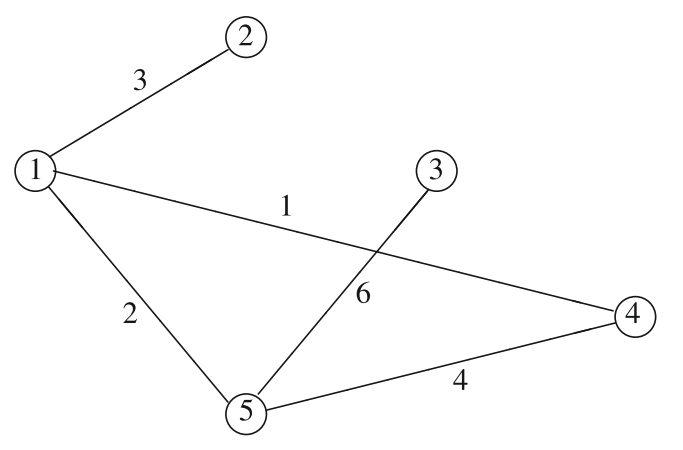
\includegraphics[scale=0.5]{1.png}
        \caption{Một đồ thị liên thông với trọng số của các cung}
        \label{fig:4.1}
    \end{figure}

    \begin{vd}
        Ta xét một đồ thị liên thông bất kỳ với các trọng số $w_{ij}$ tương ứng với cung $(i, j)$.
        Một ví dụ về đồ thị liên thông ở trong hình \ref{fig:4.1}.
        Ta xét một hạt di chuyển từ đỉnh này sang đỉnh khác theo cách sau: Nếu tại một thời điểm bất kỳ, hạt nằm ở đỉnh $i$, tiếp theo nó sẽ di chuyển đến đỉnh $j$ với xác suất $P_{ij}$ với:

        \begin{equation*}
            P_{ij} = \dfrac{w_{ij}}{\sum_j w_{ij}}
        \end{equation*}

        và $w_{ij} = 0$ nếu $(i, j)$ không phải là một cung.
        Ví dụ, với đồ thị trong hình \ref{fig:4.1}, $P_{12}=3/(3+1+2)=\dfrac{1}{2}$
    \end{vd}

    \begin{loigiai}
        Từ phương trình khả đảo thời gian:

        \begin{equation*}
            \pi_i = P_{ij} = \pi_j P_{ji}
        \end{equation*}

        trở thành:

        \begin{equation*}
            \pi_i \dfrac{w_{ij}}{\sum_j w_{ij}} = \pi_j \dfrac{w_{ji}}{\sum_i w_{ji}}
        \end{equation*}

        do $w_{ij} = w_{ji}$:

        \begin{equation*}
            \dfrac{\pi_i}{\sum_j w_{ij}} = \dfrac{\pi_j}{sum_i w_{ji}}
        \end{equation*}

        tương đương với:

        \begin{equation*}
            \dfrac{\pi_i}{\sum_j w_{ij}} = c
        \end{equation*}

        hoặc:

        \begin{equation*}
            \pi_i = c \sum_j w_{ij}
        \end{equation*}

        Vì $\sum_i \pi_i = 1$ nên:

        \begin{equation*}
            \pi_i \dfrac{\sum_j w_{ij}}{\sum_i \sum_j w_{ij}}
        \end{equation*}

        $\pi_i$ được tính từ công thức ở trên thỏa mãn điều kiện khả đảo thời gian, kéo theo quá trình là khả đảo thời gian với phân bố giới hạn.

        Với đồ thị trong hình \ref{fig:4.1}, ta có:

        \begin{equation*}
            \pi_1 = \dfrac{6}{32}, \pi_2 = \dfrac{3}{32}, \pi_3 = \dfrac{6}{32}, \pi_4 = \dfrac{5}{32}, \pi_5 = \dfrac{12}{32}
        \end{equation*}
    \end{loigiai}

    Nếu ta cố gắng giải phương trình \ref{eq:Time-Reversible} cho một xích Markov bất kỳ với các trạng thái $0, 1, \dots, M$, thường phương trình sẽ vô nghiệm.
    Ví dụ, từ phương trình \ref{eq:Time-Reversible}:

    \begin{equation*}
        \begin{aligned}
            x_i P_{ij} &= x_j P_{ji} \\
            x_k P_{kj} &= x_j P_{jk}
        \end{aligned}
    \end{equation*}

    hay (nếu $P_{ij} P_{jk} > 0$):

    \begin{equation*}
        \dfrac{x_i}{x_k} = \dfrac{P_{ji}P_{kj}}{P_{ij}P_{jk}}
    \end{equation*}

    về mặt tổng không cần bằng $P_{ki}/P_{k}$.
    Vì vậy, ta thấy điều kiện cận cho khả đảo thời gian là:

    \begin{equation} \label{eq:4.25}
        P_{ik} P_{kj} P_{ji} = P_{ij} P_{jk} P_{ki} \thickspace \forall \thickspace i, j, k
    \end{equation}

    tương đương với phát biểu sau, bắt đầu ở trạng thái $i$, dãy chuyển tiếp trạng thái $i \rightarrow k \rightarrow j \rightarrow i$ có cùng xác suất với dãy chuyển tiếp ngược $i \rightarrow j \rightarrow k \rightarrow i$.
    Để hiểu điều kiện cần, ta chú ý xác suất một dãy các bước chuyển trạng thái từ $i$ sang $k$ sang $j$ và quay lại $i$ cùng xác suất với dãy các bước chuyển trạng thái từ $i$ sang $j$ sang $k$ và sang $i$ và vì vậy ta phải có:

    \begin{equation*}
        \pi_i P_{ik} P_{kj} P_{ji} = \pi_i P_{ij} P_{jk} P_{ki}
    \end{equation*}

    với $\pi_i > 0$. Ta có thể chứng minh định lý sau:

    \begin{dl} \label{dl:4.2}
        Một xích Markov ergodic với $P_{ij}=0$ bất kỳ khi nào $P_{ji}=0$ là khả đảo thời gian khi và chỉ khi bắt đầu ở trạng thái $i$, bất kỳ quỹ đạo nào quay trở lại $i$ với xác suất bằng xác suất quỹ đạo ngược:

        \begin{equation} \label{eq:4.26}
            P_{ii_1} P_{i_1 i_2} \dots P_{i_k i} = P_{i i_k} P_{i_k i_{k-1}} \dots P_{i_1 i}
        \end{equation}

        với mọi trạng thái $i, i_1, \dots, i_k$
    \end{dl}

    \textbf{Chứng minh.}

    Ta đã chứng minh điều kiện cần.
    Để chứng minh điều kiện đủ, ta cố định trạng thái $i$ và $j$ và viết lại công thức \ref{eq:4.26} thành:

    \begin{equation*}
        P_{ii_1} P_{i_1 i_2} \dots P_{i_k j} P_{ji} = P_{ij} P_{j i_k} \dots P_{i_1 i}
    \end{equation*}

    Lấy tổng công thức trên theo tất cả các trạng thái $i_1, \dots, i_k$ ta thu được:

    \begin{equation*}
        P_{ij}^{k+1} P_{ji} = P_{ij} P_{ji}^{k+1}
    \end{equation*}

    Cho $k \rightarrow \infty$, ta thu được:

    \begin{equation*}
        \pi_j P_{ji} = P_{ij} \pi_i
    \end{equation*}

    Ta chứng minh xong định lý trên.

    \begin{vd}
        Giả sử ta được cung cấp một tập gồm $n$ phần tử, được đánh số từ 1 đến $n$ và được sắp xếp theo một danh sách có thứ tự.
        Tại từng bước thời gian, một yêu cầu truy xuất vào một trong những phần tử này, phần tử $i$ được yêu cầu (độc lập với quá khứ) với xác suất $P_i$.
        Sau khi được yêu cầu, phần tử được đặt trở lại nhưng không nhất thiết phải ở vị trí cũ.
        Thực tế, ta giả sử rằng phần tử được yêu cầu được di chuyển gần đến phía trước của danh sách hơn một bước.
        Ví dụ, nếu thứ tự trong danh sách hiện tại là 1, 3, 4, 2, 5 và phần tử 2 được yêu cầu, thứ tự mới sẽ trở thành 1, 3, 2, 4, 5.
        Ta quân tâm đến vị trí trung bình dài hạn của các phần tử được yêu cầu.
    \end{vd}

    \begin{loigiai}
        Khi được cho một vector phân bố $P=\begin{pmatrix}
            P_1, P_2, \dots, P_n
        \end{pmatrix}$, thứ tự của các phần tử có thể được mô hình hóa là một xích Markov với $n!$ trạng thái, với trạng thái tại thời điểm bất kỳ nào là thứ tự của danh sách tại thời điêm rđó.
        Ta sẽ chỉ ra rằng xích Markov này là khả đảo thời gian và sử dụng tính chất này để chỉ ra vị trí trung bình của phần tử được yêu cầu khi quy tắc di chuyển lên một bước vị trí (giả sử phần tử ở vị trí thứ hai được đẩy lên vị trí thứ nhất trong hàng) có hiệu lực nhỏ hơn so với quy luật luôn luôn di chuyển phần tử được yêu cầu lên đầu danh sách.
        Tính khả đảo thời gian của xích Markov khi quy luật di chuyển lên một bước vị trí luôn luôn dễ có hiệu lực hơn từ định lý \ref{dl:4.2}.
        Ví dụ, giả sử $n=3$ và xét đường đi từ trạng thái (1, 2, 3) quay về chính nó:

        \begin{equation*}
            (1, 2, 3) \rightarrow (2, 1, 3) \rightarrow (2, 3, 1) \rightarrow (3, 2, 1) \rightarrow(3, 1, 2) \rightarrow (1, 3, 2) \rightarrow (1, 2, 3)
        \end{equation*}

        Tích của các xác suất chuyển tiếp theo chiều thuận là:

        \begin{equation*}
            P_2 P_3 P_3 P_1 P_1 P_2 = P_1^2 P_2^2 P_3^2
        \end{equation*}

        Và xác suất chuyển tiếp theo chiều ngược là:

        \begin{equation*}
            P_3 P_3 P_2 P_2 P_2 P_2 = P_1^2 P_2^2 P_3^2
        \end{equation*}

        Bởi vì kết quả tổng quát diễn ra theo cách tương tự, xích Markov khả đảo thời gian. 
        Đối với một tham số hình thức nếu $f_i$ biểu diễn số lần phẩn tử $i$ tiến về phía trước trong quỹ đạo, khi quỹ đạo đi từ một trạng thái cố định rồi trở lại chính trạng thái này $f_i$ lần.
        Vì vậy khi quỹ đạo đảo ngược đi qua phần tử $i$ đúng bằng số lần trong quỹ đạo thuận, vì vậy tích của các xác suất chuyển trạng thái cho cả quỹ đạo thuận và quỹ đạo ngược sẽ bằng nhau và bằng:

        \begin{equation*}
            \displaystyle\prod_i P_i^{f_i + r_i}
        \end{equation*}

        với $r_i$ là số lần mà phần tử $i$ ở vị trí ban đầu và quỹ đạo thuận hoặc quỹ đạo ngược không thay đổi trạng thái.

        Với mọi hoán vị $i_1, i_2, \dots, i_n$ của $1, 2, \dots, n$, ta đặt $\pi (i_1, i_2, \dots, i_n)$ ký hiệu phân bố giới hạn ứng với quy luật dịch chuyển một vị trí.
        Với điều kiện khả đảo thời gian, ta có:

        \begin{equation} \label{eq:4.27}
            P_{i_{j+1}} \pi (i_1, \dots, i_j, i_{j+1}, \dots, i_n) = P_{i_j} \pi (i_1, \dots, i_{j+1}, i_j, \dots, i_n)
        \end{equation}

        với mọi hoán vị.

        Bây giờ ta sẽ lấy trung bình vị trí của phần tử được yêu cầu có thể được biểu diễn dưới dạng:

        \begin{equation*}
            \begin{aligned}
                \text{Vị trí trung bình } &= \displaystyle \sum_i P_i E \lbrack \text{ Vị trí của phần tử } i \rbrack \\
                &= \displaystyle \sum_i P_i \Bigg \lbrack 1+ \sum_{j \neq i} P \lbrace \text{phần tử } j \text{ đứng trước phần tử } i \rbrace \Bigg \rbrack \\
                &= 1 + \sum_i \sum_{j \neq i} P_i P \lbrace e_j \text{ đứng trước } e_i \rbrace \\
                &= \sum_{i < j} \lbrack P_i P \lbrace e_j \text{ đứng trước } e_i \rbrace + P_j P \lbrace e_i \text{ đứng trước } e_j \rbrace  \rbrack \\
                &= \sum_{i < j} \lbrack P_i P \lbrace e_j \text{ đứng trước } e_i \rbrace + P_j (1 - P \lbrace e_j \text{ đứng trước } e_i \rbrace)  \rbrack \\
                &= 1 + \sum\sum_{i<j} (P_i - P_j) P \lbrace e_j \text{ đứng trước } e_i \rbrace + \sum\sum_{i<j} P_j
            \end{aligned}
        \end{equation*}

        Vì vậy, để cực tiểu hóa vị trí trung bình của phần tử được yêu cầu, ta muốn làm cho xác suất $\lbrace e_j \text{ đứng trước } e_i \rbrace$ lớn nhất có thể khi $P_j > P_i$ và nhỏ nhất có thể khi $P_i > P_j$:

        \begin{equation*}
            P \lbrace e_j \text{ đứng trước } e_i \rbrace = \dfrac{P_j}{P_j + P_i}
        \end{equation*}

        (vì theo quy tắc đầu hàng phần tử $j$ sẽ đứng trước phần tử $i$ khi và chỉ khi yêu cầu cuối cùng cho $i$ hoặc $j$ là cho $j$).

        Vì vậy, để chỉ ra quy luật di chuyển lên một bước vị trí tốt hơn so với quy luật đầu hàng là đủ để chứng minh với luật di chuyển lên một bước:

        \begin{equation*}
            P \lbrace e_j \text{ đứng trước } e_i \rbrace > \dfrac{P_j}{P_j + P_i} \text{ khi } P_j > P_i
        \end{equation*}

        Bây giờ ta xét trạng thái bất kỳ sao cho phần tử $i$ đứng trước phần tử $j$ ví dụ $(\dots, i, i_1, \dots, i_k, j, \dots)$.
        Bằng cách chuyển vị liên tiếp các bước sử dụng công thức \ref{eq:4.27}, ta có:

        \begin{equation} \label{eq:4.28}
            \pi (\dots, i, i_1, \dots, i_k, j, \dots) = \Bigg ( \dfrac{P_i}{P_j} \Bigg)^{k+1} \pi (\dots, j, i_1, \dots, i_k, i, \dots)
        \end{equation}

        Ví dụ:

        \begin{equation*}
            \begin{aligned}
                \pi (1, 2, 3) &= \dfrac{P_2}{P_3} \pi (1, 3, 2) = \dfrac{P_2}{P_3} \dfrac{P_1}{P_3} \pi (3, 1, 2) \\
                &= \dfrac{P_2}{P_3} \dfrac{P_1}{P_3} \dfrac{P_1}{P_2} \pi (3, 2, 1) = \Bigg( \dfrac{P_1}{P_3} \Bigg)^2 \pi(3, 2, 1)
            \end{aligned}
        \end{equation*}

        Khi $P_j > P_i$, công thức \ref{eq:4.28} cho ta hiểu rằng:

        \begin{equation*}
            \pi (\dots, i, i_1, \dots, i_k, j, \dots) < \dfrac{P_i}{P_j} \pi (\dots, j, i_1, \dots, i_k, i, \dots)
        \end{equation*}

        Ta đặt $\alpha(i, j) = P \lbrace e_i \text{ đứng trước } e_j \rbrace$, ta lấy tổng tất cả các trạng thái sao cho $i$ đứng trước $j$:

        \begin{equation*}
            \alpha (i, j) < \dfrac{P_i}{P_j} \alpha (j, i)
        \end{equation*}

        Vì $\alpha(i, j) = 1 - \alpha(j, i)$, ta thu được:

        \begin{equation*}
            \alpha (j, i) > \dfrac{P_j}{P_j + P_i}
        \end{equation*}

        Vì vậy vị trí trung bình của phần tử được yêu cầu nhỏ hơn khi ở quy luật di chuyển lên một bước vị trí so với quy luật đầu hàng.    
    \end{loigiai}

    Khái niệm về xích Markov khả đảo rất hữu ích ngay cả khi quá trình là không khả đảo thời gian.
    Để minh họa, ta bắt đầu với mệnh đề sau:

    \begin{md} \label{md:4.7}
        Ta xét một xích Markov không tối giản với xác suất chuyển trạng thái $P_{ij}$.
        Nếu ta có thể tìm các số dương $\pi, i \geq 0$ và tổng bằng 1, và một ma trận xác suất chuyển tiếp $\mathbf{Q} = \lbrack Q_{ij} \rbrack$ thỏa mãn:

        \begin{equation} \label{eq:4.29}
            \pi_i P_{ij} = \pi_j Q_{ji}
        \end{equation}

        Khi đó $Q_{ij}$ là xác suất chuyển trạng thái của xích Markov ngược và $\pi_i$ là phân bố tĩnh của cả xích Markov ban đầu và xích Markov ngược.
    \end{md}

    Sự quan trọng của mệnh đề trên là ta có thể đoán đặc tính của xích Markov ngược và sử dụng hệ các phương trình ở công thức \ref{eq:4.29} để thu được phân bố tĩnh của xích Markov thuận và xích Markov và $Q_{ij}$.

    \begin{vd}
        Một bóng đèn duy nhất là đủ để thắp sáng một căn phòng.
        Khi bóng đèn bị hỏng sẽ được thay bằng một bóng đèn mới vào bắt đầu của ngày tiếp theo.
        Ta đặt $X_n$ bằng $i$ nếu bóng đèn được sử dụng vào bắt đầu của ngày thứ $n$ là ngày thứ $i$ mà bóng đèn được sử dụng (tuổi của bóng đèn là $i$).
        Ví dụ, nếu bóng đèn bị hỏng vào ngày thứ $n-1$, sau đó một bóng đèn mới được thay thế để sử dụng vào bắt đầu của ngày thứ $n$ và vì vậy $X_n = 1$.
        Ta giả sử từng bóng đèn hỏng trong ngày thứ $i$ được sử dụng với xác suất $p_i, i \geq 1$.
    \end{vd}

    \begin{loigiai}
        Ta dễ dàng thấy rằng $\lbrace X_n, n \geq 1 \rbrace$ là một xích Markov mà xác suất chuyển trạng thái được tính như sau:

        \begin{equation*}
            \begin{aligned}
                P_{i,1} &= P \lbrace \text{bóng đèn ở ngày thứ } i \text{ mà nó được sử dụng, bị hỏng} \rbrace \\
                &= P \lbrace \text{tuổi thọ bóng đèn } = i \vert \text{tuổi thọ bóng đèn } \geq 1 \rbrace \\
                &= \dfrac{P \lbrace L = i \rbrace}{P \lbrace L \geq i \rbrace}
            \end{aligned}
        \end{equation*}

        với $L$ là một biến ngẫu nhiên biểu diễn tuổi thọ của bóng đèn với $P \lbrace L = i \rbrace = p_i$. Ta nhận thấy:

        \begin{equation*}
            P_{i, i+1}=1 - P _{i, 1}
        \end{equation*}

        Ta giả sử rằng xích đã hoạt động được một thời gian dài (theo lý thuyết là vô hạn) và ta xét dãy các trạng thái đi ngược thời gian.
        Vì vậy, theo chiều thuận, trạng thái luôn tăng lên 1 đơn vị đến khi bóng đèn bị hỏng.
        Ta cũng dễ dàng thấy xích ngược luôn giảm 1 đơn vị đến khi đến 1 và sẽ nhảy lên một giá trị ngẫu nhiên biểu diễn tuổi thọ của bóng đèn trước đó.
        Vì vậy, xích ngược có xác suất chuyển trạng thái:

        \begin{equation*}
            \begin{aligned}
                Q_{i, i-1} &= 1, \thickspace i > 1 \\
                Q_{1, i} &= p_i, \thickspace i \geq 1
            \end{aligned}
        \end{equation*}

        Để kiểm tra điều này, tại cùng thời điểm xác dịnh phân bố tĩnh, ta phải thấy nếu với $Q_{ij}$ đã được cho ở công thức trên, các số dương $\lbrace p_i \rbrace$ sao cho:

        \begin{equation*}
            \pi_i P_{i, j} = \pi_j Q_{j, i}
        \end{equation*}

        Ta bắt đầu với $j=1$ và xét công thức trên:

        \begin{equation*}
            \pi_i \dfrac{P \lbrace L = i \rbrace}{P \lbrace L \geq i \rbrace} = \pi_1 P \lbrace L = i \rbrace
        \end{equation*}

        hay:

        \begin{equation*}
            \pi_i = \pi_1 P \lbrace L \geq 1 \rbrace
        \end{equation*}

        Ta lấy tổng theo $i$:

        \begin{equation*}
            1 = \sum_{i=1}^{\infty} \pi_i = \pi_1 \sum_{i=1}^{\infty} P \lbrace L \geq i \rbrace = \pi_1 E \lbrack L \rbrack
        \end{equation*}

        Và với $Q_{ij}$ biểu diễn xác suất chuyển tiếp ngược, phân bố dừng là:

        \begin{equation*}
            \pi_i = \dfrac{P \lbrace L \geq i \rbrace}{E \lbrack L \rbrack}, \thickspace i \geq 1
        \end{equation*}

        Để kết thúc chứng minh xác suất chuyển tiếp ngược và phân bố dừng như đã có ở trên, tất cả còn lại chứng minh thỏa chúng thỏa mãn:

        \begin{equation*}
            \pi_i P_{i, i+1} = \pi_{i+1} Q_{i+1, i}
        \end{equation*}

        tương đương với:

        \begin{equation*}
            \dfrac{P \lbrace L \geq 1 \rbrace}{e \lbrack L \rbrack} \Bigg (1 - \dfrac{P \lbrace L = i \rbrace}{P \lbrace L \geq 1 \rbrace} \Bigg) = \dfrac{P \lbrace L \geq i + 1 \rbrace}{E \lbrack L \rbrack}
        \end{equation*}

        Đẳng thức trên đúng do $P \lbrace L \geq i \rbrace - P \lbrace L = i \rbrace = P \lbrace L \geq i + 1 \rbrace$
    \end{loigiai}

    \section{Các phương pháp xích Markov Monte Carlo}

    Ta gọi $\mathbf{X}$ là một vector ngẫu nhiên rời rạc mà tập các giá trị có thể có là $\mathbf{x}_j, j \geq 1$.
    Ta đặt hàm trọng lượng xác suất của $\mathbf{X}$ được cho bởi $P \lbrace \mathbf{X} = \mathbf{x}_j \rbrace, j \geq 1$ và giả định rằng ta đang quan tâm việc tính đại lượng:

    \begin{equation*}
        \theta = E \lbrack h(\mathbf{X}) \rbrack = \sum_{j=1}^{\infty} h(\mathbf{x}_j) P \lbrace \mathbf{X} = \mathbf{x}_j \rbrace
    \end{equation*}

    cho từng hàm cụ thể $h$.
    Trong trường hợp việc tính toán khó khăn để tính giá trị của hàm $h(\mathbf{x}_j), j \geq 1$, ta thường chuyển sang mô phỏng để xấp xỉ $\theta$.
    Cách tiếp cận phổ biến được gọi là \textit{mô phỏng Monte Carlo}, sử dụng các số ngẫu nhiên để sinh ra một chuỗi các vector ngẫu nhiên độc lập và cùng phân bố $\mathbf{X}_1, \mathbf{X}_2, \dots, \mathbf{X}_n$ có hàm trọng lượng $P \lbrace \mathbf{X} = \mathbf{x}_j, j \geq 1$.
    Theo luật số lớn mạnh:

    \begin{equation} \label{eq:4.30}
        \lim_{n \rightarrow \infty} \sum_{i=1}^{\infty} \dfrac{h(\mathbf{X}_i)}{n} = \theta
    \end{equation}

    Vì vậy, ta có thể ước lượng $\theta$ bằng cách cho $n$ lớn và sử dụng trung bình của các giá trị của $h(\mathbf{X}_i), i=1, \dots, n$ là bộ ước lượng.

    Tuy nhiên, thường khá khó để tạo ra các vector ngẫu nhiên có hàm trọng lượng xác suất cụ thể, đặc biệt nếu $\mathbf{X}$ là một vector của các biến ngẫu nhiên phụ thuộc.
    Hơn nữa, hàm trọng lượng xác suất đôi khi được cho dưới dạng $P \lbrace \mathbf{X}=\mathbf{x}_j \rbrace = C b_j, j \geq 1$ với $b_j$ được chỉ định, nhưng $C$ phải được tính và trong nhiều ứng dụng việc tính giá trị này để cộng $b_j$ là không khả thi để xác định $C$.
    Nhưng rất may, có cách khác là sử dụng mô phỏng để ước lượng $\theta$ trong những trường hợp này.
    Bằng cách tạo ra một dãy , không là các vector độc lập nhưng các trạng thái liền kề nhau của một xích Markov với các trạng thái là vector $\mathbf{X}_1, \mathbf{X}_2, \dots$ mà phân bố dừng là $P \lbrace \mathbf{X} = \mathbf{x}_j \rbrace, j \geq 1$.
    Nếu có thể thực hiện được thì theo mệnh đề \ref{md:4.7}, phương trình \ref{eq:4.30} vẫn đúng, nghĩa là khi đó chúng ta có thể sử dụng $\sum_{i=1}^n h(\mathbf{X}_i)/n$ là một bộ ước lượng của $\theta$.

    Bây giờ ta chỉ ra bằng cách nào tạo ra một xích Markov với phân bố dừng bất kỳ có thể chỉ được chỉ định lên đến một hằng số nhân.
    Đặt $b(j), j=1, 2, \dots$ là các số thực sao cho tổng $B= \sum_{j=1}^{\infty} b(j)$ là hữu hạn.
    Cách này được gọi là \textit{thuật toán Hastings-Metropolis}, có thể được sử dụng để tạo ra xích Markov khả đảo thời gian mà phân bố dừng là:

    \begin{equation*}
        \pi (j) = b(j) / B, j = 1, 2, \dots
    \end{equation*}

    Để bắt đầu, đặt $\mathbf{Q}$ là bất kỳ một ma trận xác suất chuyển trạng thái không tối giản được chỉ định trước trên các số nguyên, với $q(i, j)$ biểu diễn phần tử hàng $i$ cột $j$ của $Q$.
    Bây giờ ta định nghĩa một xích Markov $\lbrace X_n, n \geq 0 \rbrace$ theo cách sau.
    Khi $X_n = i$, ta tạo ra một biến ngẫu nhiên $Y$ sao cho $P \lbrace Y = j \rbrace = q(i, j), j=1, 2, \dots$. Nếu $Y=j$ thì đặt $X_{n+1}$ bằng $j$ với xác suất $\alpha(i, j)$ và đặt nó bằng $i$ với xác suất $1 - \alpha(i, j)$.
    Theo các điều kiện này, dễ dàng để thấy dãy các trạng thái tạo nên một xích Markov với xác suất chuyển trạng thái $P_{ij}$ được tính bằng công thức:

    \begin{equation*}
        \begin{aligned}
            P_{ij} &= q(i, j)\alpha(i, j) \text{ nếu } j \neq i \\
            P_{ii} &= q(i, i) + \sum_{k \neq i} q(i, k)(1 - \alpha(i, k))
        \end{aligned}
    \end{equation*}

    Xích Markov này sẽ khả đảo thời gian và có phân bố dừng $\pi_j$ nếu:

    \begin{equation*}
        \pi (i) P_{i, j} = \pi_j P_{j, i} \text{ với mọi } j \neq i
    \end{equation*}

    tương đương với:

    \begin{equation} \label{eq:4.31}
        \pi (i) q(i, j) \alpha(i, j) = \pi(j) q(j, i) \alpha(j, i)
    \end{equation}

    Nhưng nếu ta lấy $\pi_j = b(j)/B$ và đặt:

    \begin{equation} \label{eq:4.32}
        \alpha(i, j) = \min \Bigg( \dfrac{\pi(j)q(j, i)}{\pi(i) q(i, j)}, 1 \Bigg)
    \end{equation}

    Khi đó công thức \ref{eq:4.31} dễ dàng thỏa mãn. Nếu:

    \begin{equation*}
        \alpha(i, j) = \min \Bigg ( \dfrac{\pi(j)q(j, i)}{\pi(i) q(i, j)}, 1 \Bigg)
    \end{equation*}

    cho ta thấy giá trị của $B$ không cần thiết để tạo ra một xích Markov, bởi vì chỉ cần giá trị $b(j)$ là đủ.
    Vậy nên hầu hết các trường hợp $\pi(j), j \geq 1$ không chỉ là phân bố dừng mà còn là phân bố giới hạn.

    \begin{vd}
        Giả sử ta muốn tạo ra một phần tử phân bố đều trong $\mathscr{S}$ là tập hợp tất cả các hoán vị $(x_1, \dots, x_n)$ của các số $(1, \dots, n)$ sao cho $\sum_{j=1}^n j x_j > a$ với $a$ là một số cho trước.
        Để tận dụng thuật toán Hastings - Metropolis ta cần định nghĩa một ma trận xác suất chuyển trạng thái của xích Markov không tối giản trong không gian trạng thái $\mathscr{S}$.
        Để thực hiện việc này, đầu tiên ta định nghĩa khái niệm các phần tử "láng giềng" của $\mathscr{S}$, và sau đó xây dựng một đồ thị mà tập các đỉnh là $\mathscr{S}$.
        Ta bắt đầu bằng đặt một cung giữa từng cặp các phần tử trong $\mathscr{S}$ mà hai hoán vị bất kỳ trong $\mathscr{S}$ được xem là các láng giềng nếu một hoán vị là kết quả từ một phép đổi chỗ của hai trong số các vị trí trong hoán vị.
        Ví dụ, $(1, 2, 3, 4)$ và $(1, 2, 4, 3)$ là các láng giềng nhưng $(1, 2, 3, 4)$ và $(1, 3, 4, 2)$ không phải láng giềng,
        
    \end{vd}

    \begin{loigiai}
        Bây giờ, ta định nghĩa một hàm xác suất chuyển trạng thái $q$ như sau: Với $N(s)$ định nghĩa là tập các láng giềng của $\mathbf{s}$ và $\lvert N (\mathbf{s}) \rvert$ bằng với số phần tử trong tập $N(\mathbf{s})$, ta đặt:
        
        \begin{equation*}
            q(\mathbf{s}, \mathbf{t}) = \dfrac{1}{\lvert N (\mathbf{s}) \rvert} \text{ nếu } t \in N(\mathbf{s})
        \end{equation*}

        Trạng thái ứng viên tiếp theo từ trạng thái $\mathbf{s}$ là một trong những trạng thái là láng giềng của $\mathbf{s}$.
        Vì phân bố giới hạn mong muốn của xích Markov là $\pi (\mathbf{s})=C$, kéo theo $\pi(\mathbf{s})=\pi(\mathbf{t})$ và vì vậy:

        \begin{equation*}
            \alpha (\mathbf{s}, \mathbf{t}) = \min(\lvert N(\mathbf{s}) \vert/ \lvert N (\mathbf{t}) \rvert, 1)
        \end{equation*}

        Nếu như trạng thái hiện tại của xích Markov là trạng thái $\mathbf{s}$ khi đó một trong số những láng giềng của trạng thái này được chọn ngẫu nhiên, giả sử là trạng thái $\mathbf{t}$.
        Nếu $\mathbf{t}$ có ít láng giềng hơn trạng thái $\mathbf{s}$ (trong lý thuyết đồ thị, bậc của đỉnh $\mathbf{t}$ nhỏ hơn bậc của đỉnh $\mathbf{s}$) khi đó trạng thái tiếp theo là $\mathbf{t}$.
        Nếu không một số ngẫu nhiên $U$ (0, 1) được sinh ra và trạng thái tiếp theo là $\mathbf{t}$ nếu $U < \lvert N(\mathbf{s}) \rvert / \lvert \mathbf{t} \rvert$ nếu không thì $\mathbf{s}$ là trạng thái tiếp theo.
        Phân bố giới hạn của xích Markov này là $\pi(\mathbf{s})=1/\lvert \mathscr{S} \rvert$ với $\lvert \mathscr{S} \rvert$ là số hoán vị (chưa biết) của $\mathscr{S}$.

    \end{loigiai}

    Phiên bản hay được sử dụng nhất của thuật toán Hastings - Metropolis là \textit{bộ lấy mẫu Gibb}.
    Đặt $\mathbf{X}=(X_1, \dots, X_n)$ là một vector ngẫu nhiên rời rạc với hàm trọng lượng xác suất $p(\mathbf{x})$ được chỉ định tối đa lên tới một hằng số nhân.
    Giả sử ta muốn tạo ra một vector ngẫu nhiên mà phân phối của $X$ đã biết.
    Ta muốn tạo ra một vector ngẫu nhiên có hàm trọng lượng:

    \begin{equation*}
        p(\mathbf{x}) = C g(\mathbf{x})
    \end{equation*}

    với $g(\mathbf{x})$ đã biết nhưng $C$ thì chưa. Việc sử dụng bộ lấy mẫu Gibb giả định với bất kỳ $i$ và giá trị $x_j, j \neq i$, ta có thể tạo ra một biến ngẫu nhiên $X$ có hàm trọng lượng xác suất:

    \begin{equation*}
        P \lbrace X = x \rbrace = P \lbrace X_i = x \vert X_j = x_j, j \neq i \rbrace
    \end{equation*}

    Cách lấy mẫu này hoạt động bằng cách sử dụng thuật toán Hastings - Metropolis trên một xích Markov với trạng thái $\mathbf{x}=(x_1, \dots, x_n)$ với một xác suất chuyển trạng thái định nghĩa như sau.
    Bất kỳ khi nào trạng thái hiện tại là $\mathbf{x}$, một tọa độ bất kỳ thuộc $1, \dots, n$ được chọn.
    Nếu tọa độ $i$ được chọn, khi đó biến ngẫu nhiên $X$ với hàm trọng lượng xác suất $P \lbrace X = x \rbrace = P \lbrace X_i = x \vert X_j = x_j, j \neq i \rbrace$ được tại ra.
    Nếu $X=x$, khi đó trạng thái $\mathbf{y}=(x_1, \dots, x_{i-1}, x, x_{i+1}, \dots, x_n)$ được xem là ứng cử viên cho trạng thái tiếp theo.
    Nói cách khác, với $\mathbf{x}$ và $\mathbf{y}$ được cho, bộ lấy mẫu Gibbs sử dụng thuật toán Hastings - Metropolis với:

    \begin{equation*}
        q(\mathbf{x}, \mathbf{y}) = \dfrac{1}{n} P \lbrace X_i = x \vert X_j = x_j, j \neq i \rbrace = \dfrac{p(\mathbf{y})}{n P \lbrace X_j = x_j, j \neq i}
    \end{equation*}

    Vì ta muốn hàm trọng lượng giới hạn là $p$, từ công thức \ref{eq:4.32} vector $\mathbf{y}$ sau đó được chấp nhận là trạng thái mới với xác suất:

    \begin{equation*}
        \begin{aligned}
            \alpha (\mathbf{x}, \mathbf{y}) &= \min \Bigg ( \dfrac{p(\mathbf{y}) q(\mathbf{y}, \mathbf{x})}{p(\mathbf{x}, q(\mathbf{x}, \mathbf{y}))}, 1 \Bigg ) \\
            &= \min \Bigg ( \dfrac{p(\mathbf{y})p(\mathbf{x})}{p(\mathbf{x})p(\mathbf{y})}, 1 \Bigg) \\
            &= 1
        \end{aligned}
    \end{equation*}
    Vì vậy, khi sử dụng bộ lấy mẫu Gibbs, các trạng thái ứng viên luôn được chấp nhận là trạng thái tiếp theo của xích.

    \begin{vd} \label{vd:4.40}
        Giả sử ta muốn tạo ra $n$ điểm phân bố đều trong hình tròn bán kính $1$ có tâm tại gốc tọa độ, với điều kiện không có hai điểm nào nằm cách một điểm khác với khoảng cách $d$.
        khi xác suất của sự kiện điều kiện này nhỏ.
        Ta có thể thực hiện sử dụng bộ lấy mẫu Gibbs như sau.
        Bắt đầu với $n$ điểm bất kỳ $\mathbf{x}_1, \dots, \mathbf{x}_n$ trong hình tròn có thuộc tính không có hai điểm trong số chúng có khoảng cách $d$ đến điểm khác, sau đó tại ra giá trị $I$ có thể là bất kỳ giá trị nào trong các giá trị $1, 2, \dots, n$.
        Sau đó ta liên tục tạo ra các điểm ngẫu nhiên trong hình tròn đến khi thu được một điểm không nằm có khoảng cách nhỏ hơn $d$ với bất kỳ đỉnh nào trong $n-1$ khác ngoại trừ $\mathbf{x}_I$.
        Tại điểm này, thay thế $\mathbf{x}_I$ bằng điểm vừa được tạo ra và lặp lại quá trình trên.
        Sau khi một lượng lớn vòng lặp của thuật toán này, tập $n$ điểm sẽ xấp xỉ có phân bố mong muốn.
    \end{vd}

    \begin{vd} \label{vd:4.41}
        Ta đặt $X_i, i = 1, \dots, n$ là các biến ngẫu nhiên độc lập tuân theo phân bố mũ với tốc độ tương ứng $\lambda_i, i = 1, \dots, n$.
        Ta đặt $S=\sum_{i=1}^n X_i$ và giả sử ta muốn sinh ra một vector ngẫu nhiên $\mathbf{X} = (X_1, \dots, X_n)$ khi có điều kiện là $S > c$ với $c$ là một hằng số dương lớn.
    \end{vd}

    \begin{loigiai}
        Ta muốn tạo ra giá trị của một vector ngẫu nhiên mà hàm mật độ là:

        \begin{equation*}
            f(x_1, \dots, x_n) = \dfrac{1}{P \lbrace S > c \rbrace} \prod_{i=1}^n \lambda_i e^{-\lambda_i x_i}, x_i \geq 0, \sum_{i=1}^n x_i > c
        \end{equation*}

        Điều này dễ thực hiện bằng cách bắt đầu với một vector $\mathbf{x}=(x_1, \dots, x_n)$ thảo mãn $x_i > 0, i=1, \dots, n, \sum_{i=1}^n x_i > c$.
        Sau đó ta tạo ra một biến ngẫu nhiên $I$ là bất kỳ giá trị nào thuộc $1, \dots, n$.
        Tiếp theo ta tạo ra một biến ngẫu nhiên tuân theo phân bố mũ $X$ với tốc độ $\lambda_I$ có điều kiện trên sự kiện $X + \sum_{j \neq I} x_j > c$.
        Bước sau, tạo ra giá trị của biến ngẫu nhiên tuân theo phân bố mũ cho biết nó vượt qua $c - \sum_{j \neq I} x_j$ được thực hiện dễ dàng bằng cách biết rằng một biến ngẫu nhiên tuân theo phân bố mũ với điều kiện lớn hơn một hằng số được phân bố là một hằng số cộng với một biến ngẫu nhiên theo phân bố mũ.
        Do đó, để thu được $X$, đầu tiên ta tạo ra một biến ngẫu nhiên theo phân bố mũ $Y$ với tốc độ $\lambda_I$ và ta đặt:\

        \begin{equation*}
            X = Y + \Bigg ( c - \sum_{j \neq I} x_j \Bigg)^+
        \end{equation*}

        với $a^+ = \max(a, 0)$

        Giá trị của $x_I$ nên được đặt lại là $X$ khi một bước lặp mới của thuật toán bắt đầu.
    \end{loigiai}

    \textbf{Lưu ý} Có thể thấy ví dụ \ref{vd:4.40} và \ref{vd:4.41} mặc dù lý thuyết cho bộ lấy mẫu Gibbs được biểu diễn giới giả định phân bố được tạo ra là rời rạc nhưng nó vẫn đúng khi phân bố là liên tục.
    
    \section{Quá trình quyết định Markov}

    Ta xét một quá trình được quan sát tại các điểm rời rạc theo thời gian có thể là một trong $M$ trạng thái có thể, ta đánh số $1, 2, \dots, M$.
    Sau khi quan sát trạng thái của quá trình, một hành động phải được chọn, ta đặt là $A$ và giả định là hữu hạn các lựa chọn, ký hiệu tập tất cả các hành động có thể.

    Nếu quá trình trong thạng thái $i$ tại thời điểm $n$ và hành động $a$ được chọn, trạng thái tiếp theo của hệ thống được xác định tuân theo xác suất chuyển trạng thái $P_{ij}(a)$.
    Nếu ta đặt $X_n$ ký hiệu là trạng thái của quá trình tại thời điểm $n$ và $x_n$ là hành động được chọn tại thời điểm $n$, khi đó tương đương với phát biểu sau:

    \begin{equation*}
        P \lbrace X_{n+1} = j \vert X_0, a_0, X_1, a_1, \dots, X_n = i, a_n = a \rbrace = P_{ij}(a)
    \end{equation*}

    Vì vậy, xác suất chuyển trạng thái là các hàm chỉ phụ thuộc vào trạng thái hiện tại và hành động kế tiếp.

    Bằng một chiến lược, ta xác định quy tắc cho việc chọn hành động.
    Ta sẽ giới hạn các chiến lược trong dạng mà các hành động mà bất kỳ lúc nào cũng chỉ phụ thuộc vào trạng thái của quá trình tại thời điểm đó (mà không phụ thuộc vào bất kỳ thông tin nào khác liên quan đến các trạng thái và hành động trước đó).T
    uy nhiên, ta sẽ cho phép chiến lược được "ngẫu nhiên hóa" trong đó các chỉ dẫn có thể là chọn các hành động bằng một phân bố xác suất.
    Hay nói cách khác, một chiến lược $\boldsymbol{\beta}$ là một tập các số $\boldsymbol{\beta}=\lbrace \beta_i (a), a \in A, i = 1, \dots, M \rbrace$ với lý giải rằng nếu quá trình ở trạng thái $i$ thì hành động $a$ được chọn với xác suất $\beta_i (a)$.
    Tất nhiên ta cần có:

    \begin{equation*}
        \begin{aligned}
            0 \leq &\beta_i (a) \leq 1, \text{ với mọi } i, a \\
            \sum_{a} &\beta_i(a) = 1, \text{ với mọi } i
        \end{aligned}
    \end{equation*}

    Với một chiến lược $\boldsymbol{\beta}$ bất kỳ đã cho, dãy các trạng thái $\lbrace X_n, n = 0, 1, \dots \rbrace$ tạo thành một xích Markov với xác suất chuyển tiếp $P_{ij} (\boldsymbol{\beta})$ được cho bởi công thức:

    \begin{equation*}
        \begin{aligned}
            P_{ij} (\boldsymbol{\beta}) &= P_{\boldsymbol{\beta}} \lbrace X_{n+1} = j \vert X_n = j \rbrace \\
            &= \sum_{a} P_{ij}(a)\beta_i (a)
        \end{aligned}
    \end{equation*}

    với đẳng thức cuối cùng có được nhờ một hệ đầy đủ các hành động được chọn khi quá trình ở trạng thái $i$.
    Ta giả định với mọi sự lựa chọn của một chiến lược $\boldsymbol{\beta}$, xích Markov kết quả là ergodic.

    Với một chiến lược $\boldsymbol{\beta}$, ta đặt $\pi_{ia}$ ký hiệu là phân bố giới hạn (hoặc trạng thái ổn định) mà quá trình khi ở trạng thái $i$ sẽ thực hiện hành động $a$ nếu chiến lược $\boldsymbol{\beta}$ được thực thi.
    Như vậy:

    \begin{equation*}
        \pi_{ia} = \lim_{n \rightarrow \infty} P_{\boldsymbol{\beta}} \lbrace X_n = i, a_n = 1 \rbrace
    \end{equation*}

    Vector $\pi = (\pi_{ia})$ phải thỏa mãn:

    \begin{equation} \label{eq:4.33}
        \begin{cases}
            \pi_{ia} \geq 0 \text{ với mọi } i, a \\
            \sum_{i} \sum_{a} \pi_{ia} = 1 \\
            \sum_a \pi_{ja} = \sum_i \sum_a \pi_{ia} P_{ij} (a) \text{ với mọi } j
        \end{cases}
    \end{equation}

    Phương trình thứ nhất và phương trình thứ hai trong \ref{eq:4.33} hiển nhiên đúng, và phương trình thứ ba là một dạng tương tự của định lý, vế trái của phương trình bằng với xác xuất trạng thái ổn định của trạng thái $j$ và vế bên phải là xác suất trạng thái ổn định của trạng thái $j$ tính theo cách lấy điều kiện trên trạng thái và hành động được chọn ở thời điểm trước.

    Vì vậy với bất kỳ chiến lược $\boldsymbol{\beta}$, có một vector $\boldsymbol{\pi}=(\pi_{ia})$ thỏa mãn hệ phương trình trên và với giải thích $\pi_{ia}$ bằng với xác suất trạng thái ổn định của trạng thái $i$ và hành động được chọn $a$ khi chiến lược $\boldsymbol{\beta}$ được sử dụng.
    Hơn nữa, ta nhận ra điều ngược lại cũng dúng.
    Cụ thể, đối với vector bất kỳ $\boldsymbol{\pi}=(\pi_{ia})$ thỏa mãn hệ phương trình trên, tồn tại một chiến lược $\boldsymbol{\beta}$ nếu $\boldsymbol{\beta}$ được sử dụng, xác suất trạng thái ổn định khi ở trạng thái $i$ và chọn hành động $a$ bằng $\pi_{ia}$.
    Để kiểm chứng điều này, ta giả sử $\boldsymbol{\pi} = (\pi_{ia})$ là một vector thỏa mãn hệ phương trình \ref{eq:4.33}.
    Ta đặt chiến lược $\boldsymbol{\beta}=(\beta_i(a))$:

    \begin{equation*}
        \begin{aligned}
            \beta_i (a) &= P \lbrace \boldsymbol{\beta} \text{ chọn } a \vert \text{ trạng thái là } i \rbrace \\
            &= \dfrac{\pi_{ia}}{\sum_a \pi_{ia}}
        \end{aligned}
    \end{equation*}

    Bây giờ ta đặt $P_{ia}$ biểu diễn phân bố giới hạn của quá trình ở trạng thái $i$ và chọn hành động $a$ khi chiến lược $\boldsymbol{\beta}$ được sử dụng.
    Ta cần chỉ ra rằng $P_{ia}=\pi_{ia}$.
    Để làm điều này ta cần chú ý $\lbrace P_{ia}, i =1, \dots, M, a \in A \rbrace$ là phân bố giới hạn của xích Markov hai chiều $\lbrace (X_n, a_n), n \geq 0 \rbrace$.
    Vì vậy, $P_{ia}$ là nghiệm duy nhất của:

    \begin{equation*}
        \begin{cases}
            P_{ia} \geq 0 \\
            \sum_i \sum_a P_{ia} = 1 \\
            P_{ja} = \sum_i \sum_{a^{\prime}}P_{ia^{\prime}}P_{ij}(a^{\prime}) \beta_j(a)
        \end{cases}
    \end{equation*}

    công thức thứ ba tính từ công thức:

    \begin{equation*}
        P \lbrace X_{n+1} = j, a_{n+1}=a \vert X_n = i, a_n = a^{\prime} \rbrace = P_{ij}(a^{\prime}) \beta_j(a)
    \end{equation*}

    Bởi vì:

    \begin{equation*}
        \beta_j (a) = \dfrac{\pi_{ja}}{\sum_a \pi_{ja}}
    \end{equation*}

    Ta nhận thấy rằng ($P_{ia}$) là nghiệm duy nhất của:

    \begin{equation*}
        \begin{cases}
            P_{ia} \geq 0 \\
            \sum_i \sum_a P_{ia} = 1 \\
            P_{ja} = \sum_i \sum_{a^{\prime}} P_{ia^{\prime}} P_{ij}(a^{\prime}) \dfrac{\pi_{ja}}{\sum_a \pi_{ja}}
        \end{cases}
    \end{equation*}
    Vì vậy, để chỉ ra $P_{ia} = \pi_{ia}$, ta cần chỉ ra:

    \begin{equation*}
        \begin{cases}
            \pi_{ia} \geq 0 \\
            \sum_i \sum_a \pi_{ia} = 1 \\
            \pi_{ja} = \sum_i \sum_{a^{\prime}} \pi_{ia^{\prime}} P_{ij} (a^{\prime}) \dfrac{\pi_{ja}}{\sum_a \pi_{ja}}
        \end{cases}
    \end{equation*}

    Hai phương trình đầu tiên suy ra từ hai phương trình đầu tiên của \ref{eq:4.33} và phương trình thứ ba tương đương với:

    \begin{equation*}
        \sum_a \pi_{ja} = \sum_i \sum_{a^{\prime}} \pi_{ia^{\prime}} P_{ij}(a^{\prime})
    \end{equation*}

    được dẫn ra từ phương trình thứ ba của \ref{eq:4.33}.

    Vì vậy ta đã chỉ ra rằng vector $\boldsymbol{\beta}=(\pi_{ia})$ thỏa mãn cả phương trình ở \ref{eq:4.33} khi và chỉ khi tồn tại một chiến lược $\boldsymbol{\beta}$ mà $\pi_{ia}$ bằng với xác suất trạng thái ổn định ở trạng thái $i$ và chọn hành động $a$ khi $\boldsymbol{\beta}$ được sử dụng.
    Thực tế chiến lược $\boldsymbol{\beta}$ được định nghĩa bằng $\boldsymbol{\beta}_i (a) = \pi_{ia} / \sum_a \pi_{ia}$.

    Các công thưc streen khá quan trọng trong việc xác định chiến lược tối ưu.
    Ví dụ, giả sử một phần thưởng $R(i, a)$ thu được khi hành động $a$ được chọn ở trạng thái $i$.
    Vì $R(X_i, a_i)$ biểu diễn phường thưởng thu được ở thời điểm $i$, phần thưởng trung bình kỳ vọng trên một đơn vị thời gian khi sử dụng chiến lược $\boldsymbol{\beta}$ được biểu diễn bằng:

    \begin{equation*}
        \text{phần thưởng trung bình kỳ vọng khi sử dụng chiến lược } \boldsymbol{\beta} = \lim_{n \rightarrow \infty} E_{\boldsymbol{\beta}} \Bigg \lbrack \dfrac{\sum_{i=1}^n R(X_i, a_i)}{n} \Bigg \rbrack
    \end{equation*}

    Nếu $\pi_{ia}$ ký hiểu xác suất trạng thái ổn định của trạng thái $i$ và chọn trạng thái $a$, phần thưởng kỳ vọng giới hạn tại thời điểm $n$:

    \begin{equation*}
        \lim_{n \rightarrow \infty} \lbrack R(X_n, a_n) \rbrack = \sum_i \sum_a \pi_{ia} R(i, a)
    \end{equation*}

    Ta có thể hiểu rằng:
    \begin{equation*}
        \text{phần thưởng trung bình kỳ vọng khi sử dụng chiến lược } \boldsymbol{\beta} = \sum_i \sum_a \pi_{ia} R(i, a)
    \end{equation*}

    Vì vậy, bài toán xác định chiến lược làm cực đại hóa phần thưởng trung bình kỳ vọng là:

    \begin{equation} \label{eq:4.34}
        \begin{aligned}
            \max_{\pi=(\pi_{ia})} &\sum_i \sum_a \pi_{ia} R(i, a) \\
            \text{ subject to } &\begin{cases} 
                                    \pi_{ia} \geq 0 \thickspace \forall i, a \\
                                    \sum_i \sum_a \pi_{ia} = 1 \\
                                    \sum_a \pi_{ja} = \sum_i \sum_a \pi_{ia} P_{ij} (a) \thickspace \forall j
                                \end{cases} 
        \end{aligned}
    \end{equation}

    Tuy nhiên bài toán cực đại hóa ở phía trên là một trường hợp đặc biệt của bài toán \textit{quy hoạch tuyến tính} và có thể được giải nhờ thuật toán quy hoạch tuyến tính tiêu chuẩn là \textit{thuật toán simplex}.
    Nếu $\boldsymbol{\beta}^* = (\pi_{ia}^*)$ cực đại hóa bài toán trên, chiến lượng tối ưu $\boldsymbol{\beta}^*$ là:

    \begin{equation*}
        \beta_i^*(a) = \dfrac{\pi_{ia}^*}{\sum_a \pi_{ia}^*}
    \end{equation*}

    \textbf{Lưu ý}

    \begin{enumerate}[label=(\roman*)]
        \item Ta có thể chỉ ra rằng $\pi^*$ làm cực đại hóa công thức \ref{eq:4.34} có đặc điểm với mỗi $i$, $\pi_{ia}^*$ bằng 0 với tất cả và chỉ bằng 1 tại $a$, ý nghĩa rằng chiến lược tối ưu là không ngẫu nhiên. Hành động mà chiến lược tối ưu quy định khi ở trạng thái $i$ là một hàm tất định của $i$.
        \item Công thức quy hoạch tuyến tính thường có hiệu quả khi có những ràng buộc. Ví dụ, giả định có một ràng buộc về tỷ lệ thời gian của quá trình ở một trạng thái nào đó, ví dụ trạng thái 1. Cụ thể, ta giả sử ta cho phép xem xét chỉ những chiến lược có đặc tính mà quý trình ở trạng thái 1 nhỏ hơn $100 \alpha$ \% của thời gian. Để xác định chiến lược tối ưu đối với yêu cầu này, ta cộng thêm vào hàm mục tiêu của bài toán quy hoạch tuyến tính ràng buộc:
        \begin{equation*}
            \sum_a \pi_{1a} \leq \alpha
        \end{equation*}

        vì $\sum_a \pi_{1a}$ biểu diễn tỷ lệ thời gian của quá trình ở trạng thái 1.
    \end{enumerate}

    \section{Xích Markov ẩn}

    Ta xét $\lbrace X_n, n = 1, 2, \dots \rbrace$ là một xích Markov với xác suất chuyển trạng thái $P_{ij}$ và xác suất trạng thái ban đầu $p_i = P \lbrace X_1 = i \rbrace, i \geq 0$.
    Ta giả sử tồn tại một tập hữu hạn $\mathscr{S}$ các tín hiệu và một tín hiệu từ $\mathscr{S}$ được phát ra tại thời điểm khi xích Markov chuyển sang một trạng thái.
    Hơn nữa, giả sử khi xích Markov chuyển sang một trạng thái $j$ khi đó tín hiệu phát ra tín hiệu $s$ với xác suất $p(s \vert j), \sum_{s \in \mathscr{S}} p(s \vert j) = 1$ độc lập với các trạng thái và tín hiệu trước đây.
    Nếu $S_n$ biểu diễn tín hiệu thứ $n$ được phát ra thì:

    \begin{equation*}
        \begin{aligned}
            P \lbrace S_1 = s \vert X_1 = j \rbrace &= p(s \vert j) \\
            P \lbrace S_n = s \vert X_1, S_1, \dots, X_{n-1}, S_{n-1}, X_n = j \rbrace &= p(s \vert j)
        \end{aligned}
    \end{equation*}

    Mô hình như trên khi dãy các tín hiệu $S_1, S_2, \dots$ được quan sát khi dãy các trạng thái xích Markov ẩn $X_1, X_2, \dots$ không được quan sát được gọi là mô hình \text{xích Markov ẩn}.

    \begin{vd} \label{vd:4.42}
        Ta xét một quá trình sản xuất mà trong từng chu kỳ có thể là trạng thái tốt (trạng thái 1) hoặc trạng thái tệ (trạng thái 2).
        Nếu quá trình ở trong trạng thái 1 thì trong suốt chu kỳ đó độc lập với quá khứ với xác suất 0.9 là trạng thái 1 ở chu kỳ tiếp theo và xác suất 0.1 là trạng thái 2.
        Khi ở trạng thái 2, quá trình sẽ ở trong trạng thái này mãi mãi.
        Ta giả sử một sản phẩm được sản xuất tại từng thời điểm và sản phẩm đó được tạo ra khi quá trình ở trạng thái 1 là đạt tiêu chuẩn chất lượng với xác suất là 0.99, từng sản phẩm được tạo ra khi quá trình ở trạng thái 2 đạt tiêu chuẩn chất lượng với xác suất 0.96.    
    \end{vd}

    \begin{loigiai}
        Với sản phẩm chấp nhận được hoặc không chấp nhận được, các sản phẩm nối tiếp nhau được sản xuất sẽ được quan sát, nhưng trạng thái của quá trình lại không quan sát được,
        vì vậy đây chính là một mô hình xích Markov ẩn.
        Tín hiệu chính là chất lượng của sản phẩm được sản xuất, có giá trị a hoặc phụ thuộc vào sản phẩm có đạt chất lượng hay không.
        Phân bố tín hiệu là:

        \begin{equation*}
            \begin{aligned}
                &p(u \vert 1) = 0.01, p(a \vert 1)=0.99, \\ &p(u \vert 2) = 0.04, p(a \vert 2) = 0.96
            \end{aligned}
        \end{equation*}

        và xác suất chuyển trạng thái của xích Markov ẩn là:

        \begin{equation*}
            P_{1, 1} = 0.9 = 1- P_{1, 2}, P_{2, 2} = 1
        \end{equation*}
    \end{loigiai}

    Mặc dù $\lbrace S_n, n \geq 1 \rbrace$ không là một xích Markov, nhưng ta cần lưu ý rằng, lấy điều kiện trên trạng thái hiện tại $X_n$, dãy $S_n, X_{n+1}, S_{n+1}, \dots$ của các trạng thái và tín hiệu ở tương lai là độc lập với dãy $X_1, S_1, \dots, X_{n-1}, S_{n-1}$ là trạng thái và tín hiệu ở quá khứ.

    Ta đặt $\mathbf{S}^n=(S_1, S_2, \dots, S_n)$ là vector ngẫu nhiên của $n$ tín hiệu ban đầu.
    Với một dãy các tín hiệu cố định $s_1, s_2, \dots, s_n$, đặt $\mathbf{s}_k = (s_1, \dots, s_k), k \leq n$.
    Để bắt đầu, ta xác định xác suất có điều kiện của xích Markov tại thời điểm $n$ khi được cho trước $\mathbf{S}^n=\mathbf{s}_n$.
    Để thu được xác suất có điều kiện này, ta đặt:

    \begin{equation*}
        F_n(j) = P \lbrace \mathbf{S}^n = \mathbf{s}_n, X_n = j \rbrace
    \end{equation*}

    và chú ý rằng:

    \begin{equation*}
        \begin{aligned}
            P \lbrace X_n = j \vert \mathbf{S}^n = \mathbf{s}_n \rbrace &= \dfrac{P \lbrace \mathbf{S}^n = \mathbf{s}_n, X_n = j}{P \lbrace \mathbf{S}^n = \mathbf{s}_n} \\
            &= \dfrac{F_n(j)}{\sum_i F_n(i)}
        \end{aligned}    
    \end{equation*}

    Bây giờ ta có:

    \begin{equation} \label{eq:4.35}
        \begin{aligned}
            F_n(j) & =P \lbrace \mathbf{S}^{n-1}=\mathbf{s}_{n-1}, S_n=s_n, X_n=j \rbrace \\
            & =\sum_i P \lbrace \mathbf{S}^{n-1}=\mathbf{s}_{n-1}, X_{n-1}=i, X_n=j, S_n=s_n \rbrace \\
            & =\sum_i F_{n-1}(i) P \lbrace X_n=j, S_n=s_n \vert \mathbf{S}^{n-1}=\mathbf{s}_{n-1}, X_{n-1}=i \rbrace \\
            & =\sum_i F_{n-1}(i) P \lbrace X_n=j, S_n=s_n \vert X_{n-1}=i \rbrace \\
            & =\sum_i F_{n-1}(i) P_{i, j} p(s_n \vert j) \\
            & =p(s_n \vert j) \sum_i F_{n-1}(i) P_{i, j}
            \end{aligned}
    \end{equation}

    với công thức trên suy ra từ công thức:

    \begin{equation*}
        \begin{aligned}
            P \lbrace X_n = j, S_n = s_n \vert X_{n-1} = i \rbrace &= P \lbrace X_n = j \vert X_{n-1} = i \rbrace \times P \lbrace S_n = s_n \vert X_n = j, X_{n-1} = i \rbrace \\
            &= P_{i, j} P \lbrace S_n = s_n \vert X_n = j \rbrace \\
            &= P_{i, j} p (s_n \vert j)
        \end{aligned}        
    \end{equation*}

    Bắt đầu với:

    \begin{equation*}
        F_1(i) = P \lbrace X_1 = i, S_1 = s_1 \rbrace = p_i p(s_1 \vert i)
    \end{equation*}

    Ta có thể sử dụng công thức \ref{eq:4.35} một cách đệ quy để xác định các hàm $F_2(i), F_3(i), \dots$ lên đến $F_n(i)$
\end{document}